 
%---------------------------------------------------------------------------
% Gui component.
%
%---------------------------------------------------------------------------


\section{GUI component}
\label{sec:arch_gui}

Write about:
- background on guis
- overall info - what it is, its role, how important guis are in general - that its an entry point for user and if sth
gets screwed here then it's affects usability 
- describe main principles - ease of use, focus on visualizations 
- dependencies,
- MVC design pattern :|
- Start analysis top down - mocks + their description
- Name logic components that will interfere with mocks (controllers, services)

Graphical user interfaces are most commonly used form of interaction with user in modern computing. Designing decent
user interface is especially important due to aim of this work - creation of application allowing measuring and
visualization of monitored processes. Although GUI component has rather limited role of giving user control over
application and allow to view results of the work it's in fact most complex component. Additionally any shortcoming in
GUI is relatively difficult to be hidden by user, and that makes UI/UX (User Interface/User Experience) engineering so
important.

During designing user interface I've been trying to follow few general principles. First of all, I wanted used
interface to be as transparent as possible. Users should focus on their tasks instead of application. Because of that,
interface shouldn't be bloated with unnecessary options and steps that users need to achieve their goals should be as
short as possible. Additionally, GUI must be coherent to free user from chaos of being spread across multiple windows,
desktops and so on. 

From business logic point of view, GUI component will extensively use MVC design pattern. Each form, window or more
complex section need to have it's own View, responsible for presentation, Controller that collects user's events and
updates view on user's actions or system events. Application will have shared model, which will be access point for
underlaying components.
 


\subsection{Architecture}

\subsection{Interface Mockups}

\begin{figure}[h]
  \centering
  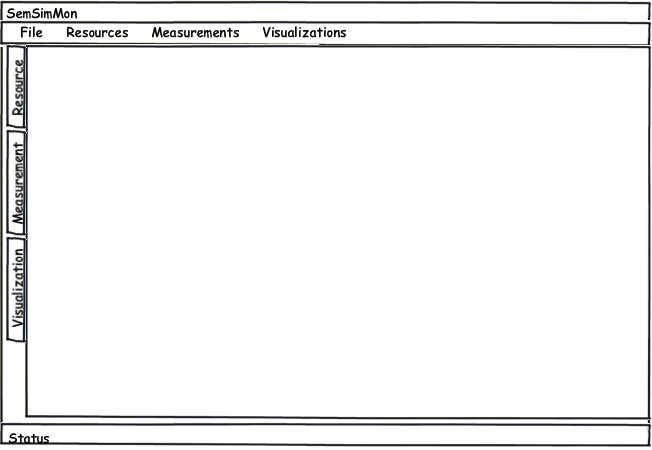
\includegraphics[width=0.7\textwidth]{mock_main}
  \caption{GUI application main view mockup}
  \label{fig:arch_overall}
\end{figure}


\begin{figure}[h]
  \centering
  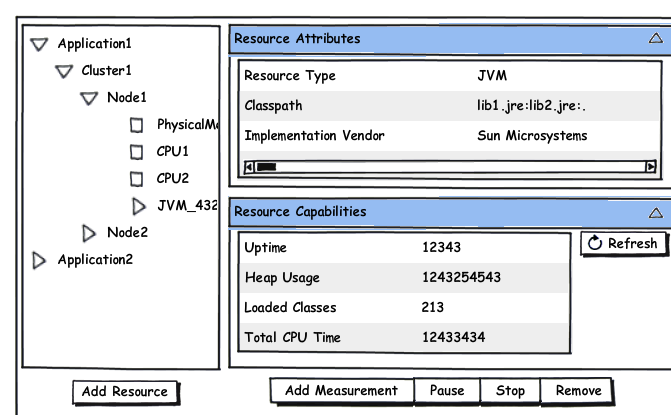
\includegraphics[width=1\textwidth]{mock_resources}
  \caption{GUI application resources pane}
  \label{fig:arch_overall}
\end{figure}

\begin{figure}[h]
  \centering
  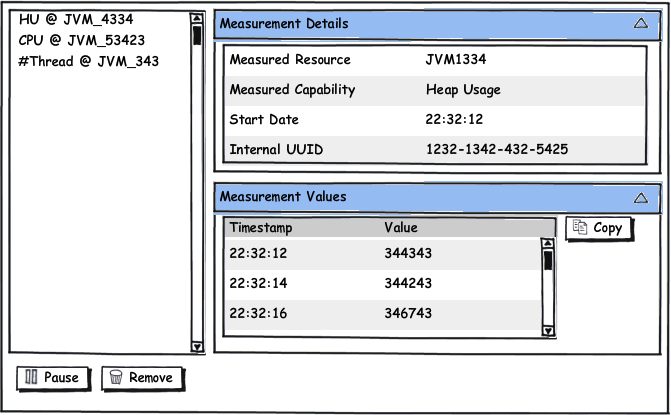
\includegraphics[width=1\textwidth]{mock_measurements}
  \caption{GUI application measurements pane}
  \label{fig:arch_overall}
\end{figure}

\begin{figure}[h]
  \centering
  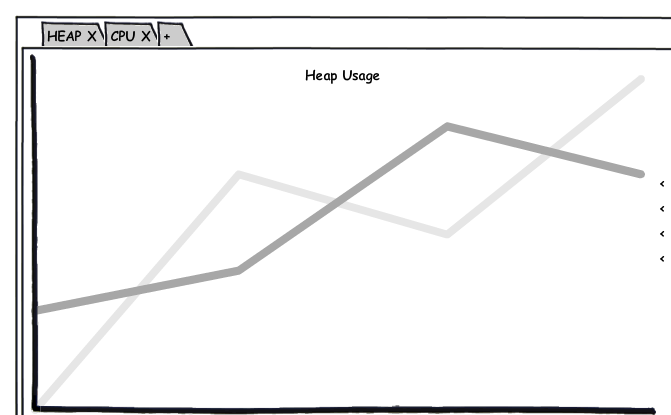
\includegraphics[width=1\textwidth]{mock_vis_clean}
  \caption{GUI application visualizations pane, clean view}
  \label{fig:arch_overall}
\end{figure}

\begin{figure}[h]
  \centering
  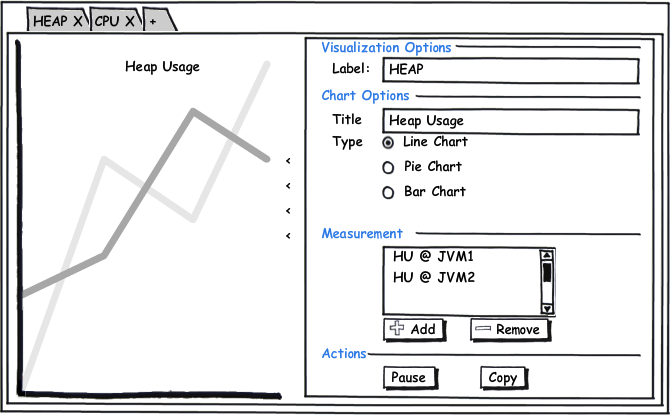
\includegraphics[width=1\textwidth]{mock_vis_options}
  \caption{GUI application visualizations pane, view with options pane}
  \label{fig:arch_overall}
\end{figure}

